\chapter{Модельно-независимое получение параметров с использованием многочастичных распадов} \label{chapt2}
В этой главе описан модельно-независимый подход к анализу многочастичных распадов (раздел~\ref{sec:dalitz}) и предложены программы исследований для симметричной Чарм-Тау-фабрики (раздел~\ref{sec:charm-tau-phenom}) и асимметричной $B$-фабрики,  а также для эксперимента \lhcb (раздел~\ref{sec:b-factory-phenom}), основанные на этом подходе.  

В пункте~\ref{sec:charm_mixing_measurement_at_ctau} описан впервые предложенный в работе автора диссертации~\cite{mixing} метод модельно-независимого измерения параметров смешивания $D$-мезонов в когерентных распадах \ddbar-пар.  В пункте~\ref{sec:time-dependent-charm-mixing} описан впервые предложенный в той же работе метод модельно-независимого измерения параметров смешивания $D$-мезонов во времязависимом анализе распадов \dkpp, который в последствии был использован для анализа данных группой \lhcb~\cite{lhcb_dkspp_mixing}.  

В пункте~\ref{sec:gamma-and-charm-mixing} рассмотрено влияние осцилляций $D$-мезонов на наблюдаемое значение параметра \gphi при модельно-независимом измерении в распадах \bdk, \dkpp и описана модификация процедуры измерения \gphi, при которой осцилляции $D$-мезонов смещают наблюдаемое значение не больше чем на $0.2\grad$, впервые предложенная в работе автора~\cite{mixing}.  
В пункте~\ref{sec:gamma-and-dcpv-in-charm} рассмотрено влияние нарушение \cpconj-симметрии в распадах \dnkpp на наблюдаемое значение параметра~\gphi при модельно-независимом измерении в распадах \bdk, \dkpp и описана модификация процедуры измерения, не предполагающая сохранение \cpconj-симметрии в распадах~\dnkpp, впервые преложенная в работе автора~\cite{bdpv_cpv}.  

В пункте~\ref{sec:model-independent-beta} описан метод модельно-независимого измерения параметра \pphi во времязависимом анализе распадов \bdsth, \dbkpp, впервые предложенный в работе автора~\cite{belle_beta_binned_dalitz}.  Первая реализация этого метода, выполненная с данными эксперимента \belle, описана в главе~\ref{sec:bdsth}.

\section{Модельно-независимый анализ трехчастичных распадов} \label{sec:dalitz}
Рассмотрение многочастичных распадов зачастую позволяет преодолеть ограничения феноменологических подходов, основанных на анализе двухчастичных распадов $B$- и $D$-мезонов.  Так, анализ трехчастичного распада $\bn\to\pi^+\pi^-\pin$ позволяет разрешить четырехкратную дискретную неопределенность при измерении параметра \aphi (пункт~\ref{sec:cpv_tree_and_loop});  $D$-мезоны из распадов \bdk, реконструированные в конечном состоянии \kspp, позволяют получить параметр \gphi (раздел~\ref{sec:cpv-phenom});  времязависимый анализ распадов \bdh, \dbkpp позволяет измерить \cosdbeta и разрешить двузначную дискретную неопределенность при измерении параметра~$2\pphi$ (раздел~\ref{sec:cpv-phenom}).  

С другой стороны, использование многочастичных распадов приводит к сложностям, связанным с ограниченным знанием динамики распада.  Амплитуда многочастичного распада является (комплексной) функцией, определенной в фазовом пространстве конечного состояния.  В отличие от модуля, комплексная фаза амплитуды многочастичного распада не может быть измерена непосредственно.  Чаще всего информацию о комплексной фазе амплитуды многочастичного распада получают исходя из модельных предположений.  
Такой подход нельзя считать удовлетворительным, поскольку он приводит к неустранимой и сложно оцениваемой неопределенности, связанной как со значением параметров модели, так и с обоснованностью применения той или иной модели.  В экспериментах с большой статистикой эти неопределенности могут стать доминирующим фактором, определяющим точность измерений.

В работе~\cite{GGSZ} была предложена идея модельно-независимого анализа распадов \dnkpp для измерения параметра \gphi в распадах \bdk.  Для измерения параметра \gphi нет необходимости знать величину \deld (уравнение~\eqref{eq:rd_deltad}) в каждой точке фазового пространства.  Достаточным является знание среднего значения $\sin\deld$ и $\cos\deld$ для нескольких областей фазового пространства.  А именно, введем параметры
\begin{equation}\label{eq:ki}
 \ki = \frac{\int\ddlzarea\left|\ad\right|^2 \ddlz}
            {\int\limits_{\mcd}\left|\ad\right|^2 \ddlz},\quad
 \kbi = \frac{\int\ddlzarea\left|\adbar\right|^2 \ddlz}
            {\int\limits_{\mcd}\left|\adbar\right|^2 \ddlz},
\end{equation}
и
\begin{equation}\label{eq:csi}
  \zi \equiv \ci + i\si = 
            \frac{\int\ddlzarea
            \left|\ad\right|\left|\adbar\right|
            e^{i\deld}\,\ddlz}
            {\int\ddlzarea\left|\ad\right|^2 \ddlz 
             \int\ddlzarea\left|\adbar\right|^2 \ddlz}
            ,
\end{equation}
где индекс $i$ обозначает номер области фазового пространства, $\mcd$ --- полное фазовое пространство и $\mcd_i$ --- область фазового пространства, соответствующую номеру~$i$.  Для параметров \ki и \kbi выполняются нормировочные условия
\begin{equation}
 \sum\limits_i \ki = 1,\quad \sum\limits_i \kbi = 1.
\end{equation}

Предполагая отсутствие \cpconj-нарушения в распадах $D$-мезонов, т.е. используя соотношение $\ad\dvar\equiv\adbar\dvarinv$, можно оптимизировать способ разбиения диаграммы Далица распада \dnkpp: выбрать $2\mcn$ области симметрично относительно перестановки $\mpsq\leftrightarrow\mmsq$.  Номера областей $i$ при этом принимают значения от $-\mcn$ до $\mcn$, исключая $0$, такие, что инверсия знаков номеров областей $i\to -i$ соответствует перестановке $\mpsq\leftrightarrow\mmsq$. При таких договоренностях выполняются соотношения
\begin{equation}\label{eq:cp-conserv-relations}
 \zi \equiv Z^*_{-i}\quad (C_i\equiv C_{-i},\quad S_i\equiv -S_{-i}),\quad \kbi \equiv \kmi.
\end{equation}

В работах~\cite{Bondar2006,Bondar2008} были изучены вопросы о том, как выбрать значение \mcn и из каких соображений выбирать форму областей.  Поясним основные выводы, полученные в этих работах, на примере измерения параметра \gphi в распадах \bdk.  Проинтегрируем уравнение~\eqref{eq:dalitz_pdf_bdk} по области $i$ и выразим результат через введенные параметры:
\begin{equation}\label{eq:dalitz_pdf_bdk_binned}
 N_i^{\pm} \propto \kmpi + \rb^2\kpmi + 2\sqrt{\ki\kmi}\left(x_{\pm}C_i+y_{\pm}S_i\right).
\end{equation}
Если неизвестные параметры \ki, \ci и \si получить из независимых измерений (способ измерения этих параметров обсуждается в пункте~\ref{sec:cs_measurement}), то из соотношений~\eqref{eq:dalitz_pdf_bdk_binned} можно получить интересующие параметры~$x_{\pm}$ и~$y_{\pm}$.

Усреднение по области фазового пространства, возникающее в результате интегрирования, приводит к уменьшению статистической чувствительности к измеряемым параметрам (в рассматриваемом случае, к параметрам $x_{\pm}$ и $y_{\pm}$).  В предельном случае большого количества областей статистическая чувствительность приближается к случаю без разбиения.  С этой точки зрения следует стремиться к увеличению количества областей.  
С другой стороны, каждая пара симметричных областей соответствует четырем неизвестным параметрам \ki, \kmi, \ci и \si; увеличение количества неизвестных параметров приводит к уменьшению статистической чувствительности к измеряемым параметрам.  В качестве эмпирического оптимального значения в настоящее время используют~$\mcn=8$.

Форма областей должна быть выбрана так, чтобы максимизировать статистическую чувствительность к измеряемым параметрам.  Хорошее приближение к оптимальному способу разбиения (смотрите уравнение~\eqref{eq:dalitz_pdf_bdk_binned}) дает критерий
\begin{equation}\label{eq:uniph}
 \frac{2\pi\left(i-\frac{1}{2}\right)}{\mcn} < \deld\dvar < \frac{2\pi\left(i+\frac{1}{2}\right)}{\mcn}\quad
 \left(\textrm{для}\ \mpsq>\mmsq\ \textrm{и}\ i>0\right).
\end{equation}
Разбиение, соответствующее этому критерию, называют \emph{равномерным по фазе}.  Критерий~\eqref{eq:uniph} может быть использован только на основе модельных соображений, поскольку функция $\deld\dvar$ неизвестна.  Важно отметить, что такое использование модели амплитуды распада не приводит к систематической ошибке измерения.  При использовании модели, плохо описывающей амплитуду распада, разбиение фазового пространства приведет, как показано в работе~\cite{Bondar2008}, только к неоптимальной статистической чувствительности к измеряемым параметрам.  
В работе~\cite{Bondar2008} также показано, что модельно-независимый подход с восемью парами областей и равномерным по фазе разбиением приводит к увеличению статистической неопределенности по сравнению с модельно-зависимым подходом примерно на $10\%$--$20\%$ (в предположении, что модель верно описывает амплитуду распада).

На рисунке~\ref{fig:binned_dalitz} показаны равномерные по фазе разбиения диаграммы Далица распада \dnkpp, полученные с помощью моделей амплитуды распада из работ~\cite{belle_gamma_dalitz_model,babar_gamma_dalitz_model}.
\begin{figure}[htb]
\begin{minipage}[b]{0.5\textwidth}
 \centering
  \includegraphics[width=0.9\textwidth]{babar_eqdel_bins}
 \subcaption{}
 \label{fig:bd_babar_eqph}
\end{minipage}
\begin{minipage}[b]{0.5\textwidth}
 \centering
  \includegraphics[width=0.9\textwidth]{belle_eqdel_bins}
 \subcaption{}
 \label{fig:bd_belle_eqph}
\end{minipage}
% \begin{minipage}[b]{0.5\textwidth}
%  \centering
%   \includegraphics[width=0.9\textwidth]{babar_opt_bins}
%  \subcaption{}
%  \label{fig:bd_babar_opt}
% \end{minipage}
% \begin{minipage}[b]{0.5\textwidth}
%  \centering
%   \includegraphics[width=0.9\textwidth]{babar_mod_bins}
%  \subcaption{}
%  \label{fig:bd_babar_mod}
% \end{minipage}
 \caption{Равномерные по фазе разбиения диаграммы Далица распада \dnkpp для моделей распада из работ а)~\cite{babar_gamma_dalitz_model} и б)~\cite{belle_gamma_dalitz_model}.}
 \label{fig:binned_dalitz}
\end{figure}

Описанный формализм может быть использован для анализа любого трехчастичного распада бесспиновой частицы на три бесспиновые частицы (например, \bdpp), в том числе для не самосопряженных распадов (например, $D^0\to K^-\pi^+\pi^0$)~\cite{mixing}.

\section{Симметричный коллайдер, работающий вблизи порога рождения пар D-мезонов} \label{sec:charm-tau-phenom}
В этом разделе рассмотрены феноменологические подходы, использующие модельно-независимый анализ трехчастичных распадов $D$-мезонов, которые могут быть использованы для анализа данных, полученных в эксперименте на Чарм-Тау-фабрике --- симметричном коллайдере с высокой светимостью, работающем вблизи порога рождения $\dn\dnbar{}^{(*)}$-пар;  показано, что подобная экспериментальная установка хорошо подходит для измерения параметров \ki, \ci и \si, а также для измерения параметров смешивания $D$-мезонов~\cite{mixing}.

\subsection{Измерение параметров \ci и \si}\label{sec:cs_measurement}
Когерентное состояние пары нейтральных $D$-мезонов, рожденных в процессе $\ep\to\ppsi\to\dn\dnbar$, аналогично состоянию пары  нейтральных $B$-мезонов, рассмотренному в пункте~\ref{sec:dt_measurements}, поскольку квантовые числа резонанса \ppsi совпадают с квантовыми числами резонанса \ups.  Предположим, что оба рожденных в таком процессе $D$-мезона перешли в конечное состояние~\kspp.  Рассмотрим интегральную по времени плотность вероятности такого процесса и возьмем необходимые для модельно-независимого подхода интегралы.  Получим:
\begin{equation}\label{eq:m_raw_asym}
 \begin{split}
  M^{\cconj-}_{ij} & \propto  \ki\kmj+ \kmi\kj - 2\sqrt{\ki\kmi\kj\kmj}\lbr\ci\cj+\si\sj\rbr\\
         &-\kj\sqrt{\ki\kmi}\lbr y_D\ci-x_D\si\rbr - \kmj\sqrt{\ki\kmi}\lbr y_D\ci+x_D\si\rbr\\
         &+\ki\sqrt{\kj\kmj}\lbr y_D\cj-x_D\sj\rbr + \kmi\sqrt{\kj\kmj}\lbr y_D\cj+x_D\sj\rbr\\
         &+\oxdydsq,
\end{split}
\end{equation}
где $i$ ($j$) обозначает номер области на диаграмме Далица распавшегося первым (вторым) $D$-мезона, $M^{\cconj-}_{ij}$ --- ожидаемую долю событий, попавших в пару областей с индексами $i$ и $j$.  В этом выражении эффект осцилляций учтен с точностью до первого порядка по параметрам смешивания включительно.  Поскольку рассматривается симметричный коллайдер, работающий вблизи порога рождения \ddbar-пар, то отлет $D$-мезонов мал и не может быть измерен, а выражение~\eqref{eq:m_raw_asym} следует усреднить по очередности распада:
\begin{equation}\label{eq:m_asym}
\begin{split}
 \left<M^{\cconj-}_{ij}\right> & \equiv \frac{1}{2}\lbr M^{\cconj-}_{ij} + M^{\cconj-}_{ji}\rbr \\
                               & \propto \ki\kmj+ \kmi\kj - 2\sqrt{\ki\kmi\kj\kmj}\lbr\ci\cj+\si\sj\rbr \\
                               & +\oxdydsq.
\end{split}
\end{equation}

Для описания случая, когда один из $D$-мезонов переходит в конечное состояние \kspp, а второй --- в состояние с определенной \cpconj-четностью $\eta_D$, в уравнении~\eqref{eq:m_asym} следует сделать формальные замены $\kj = \kmj = 1/2$, $\sj=0$ и $\cj=\eta_D$:
\begin{equation}\label{eq:m_cp_asym}
 \left<M^{\cconj-}_{i,\eta_D}\right> \propto \ki + \kmi - 2\eta_D\sqrt{\ki\kmi}C_i + \oxdydsq.
\end{equation}
В этом случае теряется чувствительность к параметрам \si.  Заметим, что мы рассматриваем параметры \ci и \si, как независимые параметры, поскольку для любой области конечного размера комбинация $\ci^2+\si^2$ не равна $1$.

Случай, когда один из $D$-мезонов переходит в состояние с определенным ароматом (например, посредством полулептонного распада $\dn\to K^-l^+\nu_l$), а второй --- в \kspp, описывается формальной заменой $\kj = 0$, $\kmj = 1$ в уравнении~\eqref{eq:m_asym}:
\begin{equation}\label{eq:m_flv_asym}
 \left<M^{\cconj-}_{i}\right> \propto \ki + \oxdydsq.
\end{equation}
Этот процесс позволяет измерить параметры \ki.

Наконец, при распаде одного $D$-мезона в адронное состояние $f_D$, такое как $K^-\pi^+$, $K^-\pi^+\pin$ и $K^-2\pi^+\pi^-$, а второго --- в состояние \kspp, необходимы формальные подстановки $\kj = \rd^2$, $\kmj = 1$, $\ci = \cos\deld$, $\si = \sin\deld$:
\begin{equation}\label{eq:m_kpi_asym}
\begin{split}
 \left<M^{\cconj-}_{i,f_D}\right> & \propto \ki + \rd^2\kmi -2\rd\sqrt{\ki\kmi}\lbr\ci\cos\deld + \si\sin\deld\rbr\\
                                  & + \oxdydsq.
\end{split}
\end{equation}

Учитывая соотношения $\left<M^{\cconj-}_{ij}\right>\equiv \left<M^{\cconj-}_{ji}\right>\equiv \left<M^{\cconj-}_{-i-j}\right>$, получаем, что соотношение~\eqref{eq:m_asym} обеспечивает $\mcn^2$ ограничений, которые позволяют определить значения $2\mcn$ неизвестных параметров \ci и \si при $\mcn\geq 2$.  Включение в анализ процессов с \cpconj-собственными распадами $D$-мезонов позволит улучшить точность измерения параметров \ci (смотрите уравнение~\eqref{eq:m_cp_asym}), а также делает систему ограничений разрешимой при $\mcn\geq 1$.  Влияние осцилляций $D$-мезонов при этом сильно подавлено и в любых мыслимых измерениях может не учитываться.  Первое измерение параметров \ci и \si было выполнено в эксперименте CLEO~\cite{CLEO_phases}.  
Измеренные значения параметров \ci и \si и соответствующие значения, полученные на основе модели амплитуды распада \dnkpp, приведены на рисунке~\ref{fig:cleo_phases}.  В настоящее время известны также предварительные результаты измерения параметров \ci и \si в эксперименте \besiii, представленные на конференции ICHEP 2016.

\begin{figure}[H]
 \centering
  \includegraphics[width=0.7\textwidth]{cleo_phases}
 \caption{Измеренные (черные круги с ошибками) и полученные из модели распада (синие звездочки) значения  параметров \ci и \si для распада \dnkpp~\cite{CLEO_phases}. (a) соответствует равномерному по фазе разбиению для модели из работы~\cite{babar_gamma_dalitz_model}, (b) соответствует разбиению, оптимизированному для измерения параметра \gphi в распадах \bdk, (c) соответствует разбиению, оптимизированному для измерения параметра \gphi в распадах \bdk с учетом фона, характерного для эксперимента LHCb, (d) соответствует равномерному по фазе разбиению для модели из работы~\cite{belle_gamma_dalitz_model}.}
 \label{fig:cleo_phases}
\end{figure}

Аналогичное рассмотрение можно выполнить, не предполагая сохранения \cpconj-симметрии в распаде \dnkpp (т.е. выполнения соотношений~\eqref{eq:cp-conserv-relations}).  Совместный анализ переходов \ddbar-пар в конечные состояния $(\kspp)_D(\kspp)_D$ и $(\kspp)_D(f_{\cpconj})_D$ в этом случае позволяет разрешить систему ограничений при $\mcn\geq 2$.  Необходимый для такого рассмотрения формализм приведен в приложении~\ref{app:full_formalism}.

%\clearpage
\subsection{Измерение параметров смешивания D-мезонов}\label{sec:charm_mixing_measurement_at_ctau}
Сокращение параметров смешивания в выражении~\eqref{eq:m_asym} произошло благодаря антисимметричности когерентного состояния нейтральных $D$-мезонов и является удачным с точки зрения измерения параметров \ci и \si.  Измерение параметров смешивания, однако, представляет отдельный интерес.  Чтобы получить чувствительность к параметрам смешивания, необходимо собрать симметричное когерентное состояние пары нейтральных $D$-мезонов.  

Оба состояния (симметричное и антисимметричное) оказываются доступными при рассмотрении процесса $\ep\to\pppsi\to\dn\dbar{}^{*0}$.  Сечение инклюзивного перехода $\ep\to\ccbar$ при энергии пучков вблизи резонанса \pppsi определяется в основном этим процессом и сравнимо с сечением вблизи резонанса \ppsi (рисунок~\ref{fig:cleo_crossection}).

\begin{figure}[htb]
 \centering
  \includegraphics[width=0.5\textwidth]{cleo_crossection_my}
 \caption{Сечения процессов $\ep\to D_{(s)}^{(*)}D_{(s)}^{(*)}(\pi)$, измеренные группой CLEO, для различных энергий~\cite{cleo_charm_crossection}.}
 \label{fig:cleo_crossection}
\end{figure}

\cconj-четность пары $D$-мезонов определяет мода распада $\dstn$-мезона: при распаде $\dstn\to\dn\gamma$ пара $D$-мезонов переходит в симметричное состояние с $\cconj=+1$, а при распаде $\dstn\to\dn\pin$ --- в антисимметричное состояние с $\cconj=-1$.  Второй случай был рассмотрен в пункте~\ref{sec:cs_measurement}.  Рассмотрим здесь первый случай и начнем с перехода обоих $D$-мезонов в конечное состояние \kspp.  Доля событий, попавших в пару областей с номерами $(i,j)$, задается выражением
\begin{equation}\label{eq:m_sym}
\begin{split}
  \left<M^{\cconj+}_{ij}\right> 
  & \propto \ki\kmj+\kmi\kj + 2\sqrt{\ki\kmi\kj\kmj}\lbr\ci\cj+\si\sj\rbr \\
  & + 2\kj\sqrt{\ki\kmi}\lbr y_D\ci-x_D\si\rbr + 2\kmj\sqrt{\ki\kmi}\lbr y_D\ci+x_D\si\rbr \\
  & + 2\ki\sqrt{\kj\kmj}\lbr y_D\cj-x_D\sj\rbr + 2\kmi\sqrt{\kj\kmj}\lbr y_D\cj+x_D\sj\rbr \\
  & + \oxdydsq.
\end{split}
\end{equation}
Заметим, что линейный по параметрам смешивания вклад удваивается при усреднении по очередности распада.  Выпишем выражения, соответствующие симметричному когерентному состоянию пары нейтральных $D$-мезонов, для тех же случаев, что были рассмотрены в пункте~\ref{sec:cs_measurement}:
\begin{itemize}
 \item Один из $D$-мезонов распадается в состояние с определенной \cpconj-четностью $\eta_D$:
 \begin{equation}\label{eq:m_cp_sym}
  \begin{split}
   \left<M^{\cconj+}_{i,\eta_D}\right> 
  & \propto \lbr\ki+\kmi\rbr\lbr1 + 2\eta_D y_D\rbr + 2\ci\sqrt{\ki\kmi}\lbr\eta_D + 2y_D\rbr \\
  & + \oxdydsq.
  \end{split}
 \end{equation}
 \item Один из $D$-мезонов распадается в состояние с определенным ароматом:
 \begin{equation}\label{eq:m_flv_sym}
  \left<M^{\cconj+}_{i}\right> 
  \propto \ki + 2\sqrt{\ki\kmi}\lbr y_D\ci+x_D\si\rbr + \oxdydsq.
 \end{equation}
 \item Один из $D$-мезонов распадается в адронное состояние ($f_D = K^-\pi^+$ и другие):
 \begin{equation}\label{eq:m_kpi_sym}
\begin{split}
  \left<M^{\cconj+}_{i,f_D}\right> 
  & \propto \ki+\kmi\rd^2 + 2\rd\sqrt{\ki\kmi}\lbr\ci\cos\deld+\si\sin\deld\rbr \\
  & + 2\sqrt{\ki\kmi}\lbr y_D\ci+x_D\si\rbr + \oxdydsq.
\end{split}
\end{equation}
\end{itemize}

Процесс $\pppsi\to D^{\pm}D^{*\mp}$, \dstpdpip, \dnkpp позволяет получить нейтральный $D$-мезон в некогерентном состоянии.  Используя уравнения~\eqref{eq:flavor_states_evolution} и~\eqref{eq:kap_sig_d}, можно получить интегральную по времени вероятность обнаружить событие в области диаграммы Далица с индексом $i$:
\begin{equation}\label{eq:kprime}
 \ki^{\prime} = \ki + \sqrt{\ki\kmi}\lbr y_D\ci + x_D\si\rbr + \oxdydsq.
\end{equation}
Способ получения параметров \ki, \ci и \si обсуждался в пункте~\ref{sec:cs_measurement}.  При известных значения этих параметров соотношения~\eqref{eq:m_cp_sym}, \eqref{eq:m_flv_sym} и \eqref{eq:kprime} позволяют получить параметры смешивания $x_D$ и $y_D$.

\paragraph{Обобщение на другие многочастичные распады $D$-мезонов. } Параметры смешивания могут быть измерены с использованием таких трех- и четырехчастичных конечных состояний $D$-мезона, как \kppn и $K^-2\pi^+\pi^-$.  Для разрешенного $\dn\to\kppn$ и подавленного $\dn\to K^+\pi^-\pin$ распадов можно определить параметры \ki, \ci и \si аналогично~\eqref{eq:ki} и~\eqref{eq:csi}.  Относительная величина интерференционного слагаемого при использовании этих процессов может быть гораздо большей, чем при использовании распадов \dkpp.  Например, если один из пары $D$-мезонов, находящихся в когерентном состоянии с $\cconj=+1$, распадается полулептонно, как \dn-мезон, а второй --- в конечное состояние \kppn (состояние с \emph{неверным знаком}), то мы приходим к случаю, описываемому уравнением~\eqref{eq:m_flv_sym}, причем первое слагаемое имеет величину порядка $r_{\kppn} \sim 0.06\times 0.06$, а второе --- $\sqrt{r_{\kppn}}(x_D,y_D)\sim 0.06\times 0.01$.

Динамика разрешенного распада $\dn\to\kppn$ была изучена в работе~\cite{CLEO_kpipi0}, а подавленного $\dnbar\to\kppn$ --- в работе~\cite{babar_ws_kpipi0}.  На основе этих результатов мы получили равномерное по фазе разбиение диаграмм Далица для этих распадов (рисунок~\ref{fig:kpipin_binning}) и значения параметров \ki, \ci и \si, которые используются в описанной ниже оценке точности измерения параметров смешивания.

\begin{figure}[htb]
 \centering
  \includegraphics[angle=90,width=0.45\textwidth]{Kpipi0Binning2}
 \caption{Равномерное по фазе разбиение диаграммы Далица распадов $D\to\kppn$, полученное с помощью моделей амплитуд распадов из работ~\cite{CLEO_kpipi0,babar_ws_kpipi0}.}
 \label{fig:kpipin_binning}
\end{figure}

\paragraph{Количественная оценка точности измерения параметров смешивания на Чарм-Тау-фабрике. }
Одна из возможных схем измерения параметров смешивания на Чарм-Тау-фабрике, работающей вблизи резонанса \pppsi, состоит в использовании
\begin{enumerate}
 \item многочастичных распадов $D$-мезонов, рождающихся в когерентном состоянии с определенным ароматом и $\cconj=-1$ (уравнение~\eqref{eq:m_flv_asym});
 \item распадов пары $D$-мезонов, рождающихся в когерентном состоянии с $\cconj=-1$, в одно и то же многочастичное состояние (уравнение~\eqref{eq:m_asym});
 \item многочастичных распадов $D$, рождающихся в некогерентном состоянии с определенным ароматом (уравнение~\eqref{eq:kprime});
 \item многочастичных распадов $D$, рождающихся в когерентном состоянии с определенным ароматом и $\cconj=+1$ (уравнение~\eqref{eq:m_flv_sym}).
\end{enumerate}
Первый тип распадов позволяет измерить параметры \ki, второй --- параметры \ci и \si, третий и четвертый типы чувствительны к параметрам смешивания.

В таблице~\ref{tab:EvNum_Step} приведена оценка количества событий перечисленных типов для конечных состояний \kspp и \kppn, соответствующая году работы Чарм-Тау-фабрики со светимостью $10^{35}\lumi$.  Проекты таких установок обсуждаются~\cite{Levichev2008}.  

\begin{table}
\begin{center}
\caption{Оценка количества зарегистрированных распадов $D$ в конечные состояния \kspp и \kppn, соответствующая году работы Чарм-Тау-фабрики со светимостью $10^{35}\lumi$, работающей вблизи резонанса \pppsi.  Эффективность регистрации событий оценена на основе результатов группы CLEO~\cite{CLEO_phases}.  Значения для конечного состояния \kppn включают разрешенные и подавленные переходы.}
\label{tab:EvNum_Step}
\begin{tabular}{ccc}\hline\hline
\multirow{2}{*}{Тип процесса} & \multicolumn{2}{c}{Количество событий ($10^6$)} \\ %\cline{2-3}
& \kspp & \kppn \\ \hline
Некогерентные с определенным ароматом         & $6$   & $30$  \\
Когерентные $\cconj-$ с определенным ароматом & $2.1$ & $10.5$\\
Когерентные $\cconj+$ с определенным ароматом & $1.4$ & $ 7$  \\
Когерентные $\cconj-$                         & $0.6$ & $13$  \\
\hline\hline
\end{tabular}
\end{center}
\end{table}

Используя полученные оценки размера выборок, мы выполнили серию численных экспериментов методом Монте-Карло (описание процедуры приведено в приложении~\ref{app:toy-mc}) для оценки статистической неопределенности при измерении параметров смешивания по описанной схеме.   При проведении численных экспериментов использованы модели амплитуд распадов \dnkpp из работы~\cite{belle_gamma_dalitz_model}, распадов $\dn\to \kppn$ из работы~\cite{CLEO_kpipi0} и распадов $\dnbar\to\kppn$ из работы~\cite{babar_ws_kpipi0}.  Результаты оценок представлены в таблицах~\ref{tab:Mix_Error} и~\ref{tab:Mix_Error_Kpipi0}.  Кроме параметров смешивания $x_D$ и $y_D$, в таблицах приведены оценки статистической неопределенности для параметров $\alpha_{\cpconj}$ и $r_{\cpconj}$, описывающих \cpconj-нарушение в смешивании $D$-мезонов:
\begin{equation}
 r_{\cpconj} e^{i\alpha_{\cpconj}}\equiv \frac{p}{q},
\end{equation}
где $p$ и $q$ определены в уравнении~\eqref{eq:basis_transformation}.  Для наглядности, мы не учитывали возможное нарушение \cpconj-симметрии в осцилляциях $D$-мезонов при описании формализма.  Необходимое расширение формализма приведено в работах~\cite{mixing,xing} и в приложении~\ref{app:full_formalism}.  Полученные оценки показывают, что в эксперименте на Чарм-Тау-фабрике параметры смешивания $D$-мезонов могут быть измерены с точностью лучше $10^{-3}$.  Существующие, модельно-зависимые, измерения параметров смешивания на $B$-фабриках~\cite{peng_mixing,babar_dkspp_mixing} имеют статистическую неопределенность около $2\times 10^{-3}$.

\begin{table}
\begin{center}
\caption{Результат численных экспериментов: статистическая неопределенность при модельно-независимом измерении параметров смешивания и \cpconj-нарушения в смешивании $D$-мезонов с использованием переходов $D$-мезонов в конечное состояние \dkpp.  Результат соответствует году работы Чарм-Тау-фабрики со светимостью $10^{35}\lumi$, работающей вблизи резонанса \pppsi.  Для выполнения численных экспериментов использована модель амплитуды распада \dnkpp из работы~\cite{belle_gamma_dalitz_model}.}
\label{tab:Mix_Error}
\begin{tabular}{lccc}\hline\hline
\multirow{2}{*}{Параметр} & \multicolumn{3}{c}{Статистическая неопределенность} \\ %\cline{2-4}
&Когерентные события&Некогерентные события&Все события\\ \hline
$x_D$ ($10^{-4}$)  			& $12.5$ & $18.4$ & $11.8$ \\
$y_D$ ($10^{-4}$)  			& $ 8.7$ & $12.9$ & $8.5$  \\
$r_{\cpconj}$ ($10^{-2}$)     		& $ 5.4$ & $ 5.2$ & $3.8$  \\
$\alpha_{\cpconj}$ (град.) 		& $ 3.5$ & $ 3.5$ & $2.5$  \\ 
\hline\hline
\end{tabular}
\end{center}
\end{table}

\begin{table}
\begin{center}
\caption{Результат численных экспериментов: статистическая неопределенность при модельно-независимом измерении параметров смешивания и \cpconj-нарушения в смешивании $D$-мезонов с использованием переходов $D$-мезонов в конечное состояние \kppn.  Результат соответствует году работы Чарм-Тау-фабрики со светимостью $10^{35}\lumi$, работающей вблизи резонанса \pppsi.  Для выполнения численных экспериментов использованы модели амплитуд распадов $\dn\to\kppn$ из работы~\cite{CLEO_kpipi0} и распадов $\dnbar\to\kppn$ из работы~\cite{babar_ws_kpipi0}, а также значение $\deld^{K\pi\pin}=227\grad$ средней разности фаз между амплитудами распадов $\dn\to\kppn$ и $\dnbar\to\kppn$, из работы~\cite{CLEO_kpipi0}.}
\label{tab:Mix_Error_Kpipi0}
\begin{tabular}{lccc}\hline\hline
\multirow{2}{*}{Параметр} & \multicolumn{3}{c}{Статистическая неопределенность} \\% \cline{2-4}
&Когерентные события&Некогерентные события&Все события\\ \hline
$x_D$ ($10^{-4}$)  		& $6.2$ & $8.7$ & $6.0$ \\
$y_D$ ($10^{-4}$)  		& $6.1$ & $8.9$ & $6.1$ \\
$r_{\cpconj}$ ($10^{-2}$)     	& $2.6$ & $2.2$ & $1.7$ \\
$\alpha_{\cpconj}$ (град.) 	& $2.4$ & $2.4$ & $1.7$  \\ 
\hline\hline
\end{tabular}
\end{center}
\end{table}

\paragraph{Обсуждение метода. } При развитии формализма мы предполагали отсутствие прямого \cpconj-нарушения в распадах $D$-мезонов.  Возможное прямое \cpconj-нарушение может быть включено в формализм посредством удвоения количества параметров \ki, \ci и \si: в этом случае необходимо рассматривать два набора параметров для каждого аромата $D$ (смотрите пункт~\ref{sec:gamma-and-dcpv-in-charm}).  Количество ограничений (уравнений) при этом остается неизменным, а система уравнений остается разрешимой при достаточно большом количестве областей на диаграмме Далица.  Такой, обобщенный, формализм позволяет различать прямое \cpconj-нарушение в распадах $D$-мезонов и \cpconj-нарушение в осцилляциях.

\cpconj-нарушение в системе нейтральных $K$-мезонов может имитировать \cpconj-нарушение в системе нейтральных $D$-мезонов, если используется конечное состояние \kspp или другое, содержащее \ks-мезон.  \cpconj-нарушающие слагаемые в амплитуде распада $D$-мезона порядка $\epsilon\lambda^2$, где $\epsilon\approx 2.2\times 10^{-3}$~\cite{pdg} --- величина \cpconj-нарушения в смешивании $K$-мезонов и $\lambda^2\approx0.04$ (уравнение~\eqref{eq:wolf_param_values}) описывает относительную разницу между амплитудами распадов \dnkpp и $\dn\to K_L^0\pi^+\pi^-$.  Величина наблюдаемого \cpconj-нарушения составит порядка $r_{\cpconj}\sim \epsilon\lambda^2/(x_D+y_D)^2\sim 0.01$.  Зная структуру амплитуды распада $\dn\to K_L^0\pi^+\pi^-$ (такого рода анализ также может быть выполнен на Чарм-Тау-фабрике), в измерения можно ввести поправку, компенсирующую описанный эффект.

Существенным свойством описанного подхода является возможность получения всей необходимой информации в одном эксперименте, в измерениях со схожей кинематикой.  Это позволяет рассчитывать на значительное сокращение систематических эффектов, связанных с эффективностью регистрации частиц.  Кроме того, для получения значений всех параметров необходимы измерения только относительных величин --- долей событий в областях диаграммы Далица, что также позволяет ожидать избавления от некоторых систематические неопределенностей, связанных с эффективностью реконструкции событий.

Оптимальной энергией пучков симметричной Чарм-Тау-фабрики для реализации представленной программы измерений является $\sqrt{s}=4.01\gev$.  Это значение находится под порогом рождения пар $D^*\dbar{}^{*}$, распады которых могут являться существенным источником фона для распадов пар $D\dbar{}^{*}$, а сечение процесса $\ep\to D\dbar{}^{*}$ при этой энергии все еще достаточно велико (смотрите рисунок~\ref{fig:cleo_crossection}).

\section{Асимметричный коллайдер, работающий вблизи порога рождения пар B-мезонов} \label{sec:b-factory-phenom}
В этом разделе рассмотрена феноменология модельно-независимых измерений с использованием многочастичных распадов на асимметричном ускорителе с высокой светимостью, работающем вблизи энергии резонанса \ups ($B$-фабрике)~\cite{mixing,bdpv_cpv}.  Описанные методы измерений также могут быть использованы в эксперименте LHCb.

\subsection{Измерение параметров смешивания D-мезонов во времязависимом анализе}\label{sec:time-dependent-charm-mixing} \label{sec:charm_mixing_measurement_at_bfac}
Временная эволюция нейтральных $D$-мезонов обсуждалась в разделе~\ref{sec:mixing}.  Уравнения~\eqref{eq:flavor_states_evolution} и~\eqref{eq:kap_sig_d} позволяют получить времязависимую плотность вероятности распада \dn-мезона.  Рассматривая переход в конечное состояние \kspp и интегрируя по области диаграммы Далица с индексом $i$, получим
\begin{equation}\label{eq:kprime-time}
 \ki^{\prime}\lbr t\rbr \propto \dexp\left[ \ki+\sqrt{\ki\kmi}\lbr y_D\ci+x_D\si\rbr\Gamma t+ \oxdydtsq \right].
\end{equation}
Уравнение~\ref{eq:kprime-time} может быть использовано для модельно-независимого измерения параметров смешивания $D$-мезонов.  В приложении~\ref{app:full_formalism} приведен более общий формализм, учитывающий возможное нарушения \cpconj-симметрии в осцилляциях $D$-мезонов.  Расширенный формализм позволяет выполнять модельно-независимые измерения параметров \cpconj-нарушения в осцилляциях $D$-мезонов совместно с параметрами смешивания.  

Данный метод впервые описан в работе~\cite{mixing} и впоследствии впервые реализован группой \lhcb в работе~\cite{lhcb_dkspp_mixing}, в которой представлен анализ $178\times 10^3$ распадов \dstpdpip, \dnkpp.  Существуют планы по проведению аналогичного анализа с данными экспериментов Belle и BaBar, которые набрали около $10^6$ распадов \dstpdpip, \dnkpp.  Описанный метод вероятно будет востребован при проведении измерений с большей статистикой с данными эксперимента \belleii.

\subsection{Влияние осцилляций D-мезонов на модельно-независимое измерение параметра \gphi}\label{sec:gamma-and-charm-mixing}
В пункте~\ref{sec:dalitz} обсуждалось модельно-независимое измерение параметра \gphi в распадах \bdk, \dkpp (уравнение~\eqref{eq:dalitz_pdf_bdk_binned}).  В перспективе прецизионного модельно-независимого измерения параметра \gphi в экспериментах \belleii и \lhcb важным вопросом является возможное влияние осцилляций $D$-мезонов на наблюдаемую величину \gphi.  Выражение~\eqref{eq:dalitz_pdf_bdk_binned} с учетом осцилляций $D$-мезонов принимает вид
\begin{equation}\label{eq:n_mix}
  \begin{split}
   N^{\pm\prime}_i 
    & \propto \kpmi + \rb^2\kmpi + 2\sqrt{\ki\kmi}\lbr x_{\pm}\ci+y_{\pm}\si\rbr \\
    & +\sqrt{\ki\kmi}\lbr y_D\ci+x_D\si\rbr + \rb^2\sqrt{\ki\kmi}\lbr y_D\ci-x_D\si\rbr\\
    & + \kpmi\lbr x_{\pm}y_D-y_{\pm}x_D\rbr + \kmpi\lbr x_{\pm}y_D+y_{\pm}x_D\rbr+\oxdydsq. 
  \end{split}
\end{equation}

Значения параметров \ki, \ci и \si, измеренные на Чарм-Тау-фабрике с использованием процесса $\ep\to\ppsi\to\dn\dnbar$ не подвержены влиянию осцилляций $D$-мезонов с точностью до поправок второго порядка по параметрам смешивания (пункт~\ref{sec:cs_measurement}).  Если использовать измеренные таким образом значения \ki, \ci и \si для извлечения параметра~\gphi и не учитывать эффект осцилляций $D$-мезонов, то систематический сдвиг за счет осцилляций будет линейным по параметрам смешивания.

Другим возможным выбором является использование значений параметров \ki, измеренных в некогерентных распадах \dstpdpip, \dnkpp (уравнение~\eqref{eq:kprime}), и поэтому искаженных осцилляциями $D$-мезонов в первом порядке по параметрам смешивания.  Для анализа этого случая уравнение~\eqref{eq:n_mix} удобно переписать в виде~\cite{mixing}
\begin{equation}\label{eq:n_mix_k_mix}
  N^{\pm\prime}_i = 
    \kpmipr + \rb^2\kmpipr + 2\sqrt{\kipr\kmipr}\lbr x_{\pm}\cipr+y_{\pm} \sipr\rbr+\oxdydsq
  \,, 
\end{equation}
где \kipr определены в уравнении~\eqref{eq:kprime},
\begin{equation}
\begin{split}
  \cipr = \ci & + \kppkpovkpkp \lbr 1-\ci^2\rbr y_D
               + \kpmkpovkpkp \ci\si x_D, \\
  \sipr = \si & - \kpmkpovkpkp \lbr 1-\ci^2\rbr x_D
               - \kppkpovkpkp \ci\si y_D.
\end{split}
\end{equation}
Параметры \cipr и \sipr отличаются от параметров \ci и \si линейными по параметрам смешивания поправками, а уравнение~\eqref{eq:n_mix_k_mix} имеет тот же вид, что уравнение~\eqref{eq:dalitz_pdf_bdk_binned}.  Линейный по параметрам смешивания вклад в уравнении~\eqref{eq:n_mix_k_mix} дополнительно подавлен фактором порядка \rb по сравнению с соответствующим вкладом в уравнении~\eqref{eq:n_mix}.  Это позволяет ожидать, что смещение наблюдаемого значения \gphi в случае получения параметров \ki в некогерентных распадах будет значительно меньше соответствующего смещения в случае получения параметров \ki в когерентных распадах.

Заметим, что несмещенное значение \gphi (с точностью до поправок второго порядка по параметрам смешивания) можно получить, если значения параметров \ki определять в некогерентных распадах, а значения параметров \cipr и \sipr определять вместе со значениями параметров $x_B$ и $y_B$ из соотношений~\eqref{eq:n_mix_k_mix}.  В этом случае, однако, статистическая чувствительность к параметрам $x_B$ и $y_B$ значительно уменьшается.  

Количественная оценка влияния осцилляций $D$-мезонов на наблюдаемое значение параметра \gphi была выполнена с помощью численных экспериментов Монте-Карло.  При этом значения параметров \ki, \ci и \si вычислялись с помощью модели распада \dnkpp из работы~\cite{belle_gamma_dalitz_model} и рассматривались три схемы измерения:
\begin{enumerate}
 \item Использование значений параметров \ki, \ci и \si, измеренных в когерентных распадах $D$-мезонов.
 \item Использование значений параметров \ci и \si, измеренных в когерентных распадах $D$-мезонов, а значения параметров \ki --- в некогерентных распадах (\kipr).
 \item Использование значений параметров \ki, \ci и \si, измеренных в когерентных распадах $D$-мезонов и применение линейной поправки согласно уравнению~\eqref{eq:n_mix} (считая параметры смешивания известными).
\end{enumerate}
Величина поправки к наблюдаемой величине параметра \gphi за счет осцилляций $D$-мезонов зависит от величины $\alpha_D=\arctan(y_D/x_D)$, отношения $\sqrt{x_D^2+y_D^2}/r_B$ и значений параметров \delb и \gphi.  Мы выбрали значение $\sqrt{x_D^2+y_D^2}/r_B=0.1$ (поправка линейна по этому параметру) и выполнили сканирование по остальным параметрам.  Результаты приведены в таблице~\ref{tab:Gamma_bias} и показывают, что использование значений параметров \ki, полученных из некогерентных распадов $D$-мезонов, позволяет уменьшить влияние осцилляций $D$-мезонов до пренебрежимого на практике значения.
\begin{table}[H]
\begin{center}
\caption{Результаты численных экспериментов: смещения наблюдаемого значения параметра \gphi при модельно-независимом измерении в распадах \bdk, \dkpp, возникающие из-за осцилляций $D$-мезонов.  Приведены максимальные смещения \gphi, полученные при сканировании по параметрам $\alpha_{D}=\arctan(y_D/x_D)$, $\delta_B$ и \gphi, а также значения параметров, при которых эти смещения были получены.  Смещения пропорциональны величине $\sqrt{x_D^2+y_D^2}/r_B$, приведенные значения соответствуют значению $0.1$.}
\label{tab:Gamma_bias}
\begin{tabular}{lcccc}
\hline\hline 
Схема измерения        &$\Delta\gphi_{\textrm{max}}$&$\alpha_{D,\textrm{max}}$&$\delta_{B,
\rm max}$&$\gamma_{B, \textrm{max}}$\\ 
\hline 
1. Использование \ki   &$ 2.9 \grad$ &$184\grad$ &$85\grad$ &$87\grad$\\ 
2. Использование \kipr &$-0.2 \grad$ &$ 97\grad$ &$ 2\grad$ &$90\grad$\\ 
3. Линейная поправка   &$ 0.07\grad$ &$324\grad$ &$72\grad$ &$73\grad$\\ 
\hline\hline 
\end{tabular}
\end{center}
\end{table}

\subsection{Влияние прямого CP-нарушения в распадах D-мезонов на модельно-независимое измерение параметра \gphi}\label{sec:gamma-and-dcpv-in-charm}
Прецизионные измерения параметра \gphi в экспериментах \lhcb и \belleii могут выявить отклонения от \km-механизма.  В этом случае важно будет понимать природу этого отклонения: проявление ли это эффектов НФ в распадах $B$-мезонов или $D$-мезонов?  В этом пункте описывается оценка возможного систематического смещения наблюдаемой величины параметра \gphi из-за прямого \cpconj-нарушения в распадах \dkpp с учетом существующих экспериментальных ограничений на его величину.  Также показывается, что модельно-независимый подход может быть применен и в случае существования прямого \cpconj-нарушения в распадах $D$-мезонов, позволяя получать несмещенные измерения при незначительном уменьшении статистической чувствительности метода~\cite{bdpv_cpv}.

Допуская \cpconj-нарушение в распаде \dkpp, нельзя предполагать выполнение соотношения $\ad\dvar\equiv\adbar\dvarinv$.  Тогда, вообще говоря,
\begin{equation}
 \kbi\neq \kmi,\quad
 \ci\neq C_{-i},\quad
 \si\neq -S_{-i}.
\end{equation}
Симметричность разбиения диаграммы Далица в этом случае теряет практическую ценность, а количество независимых параметров \ki, \kbi, \ci и \si удваивается.    

Запишем выражения для ожидаемых долей чисел событий в областях диаграммы Далица для процессов, используемых при модельно-независимом измерении параметра \gphi, не предполагая сохранение \cpconj-симметрии в распаде \dnkpp.  Уравнение~\eqref{eq:m_cp_asym} перейдет в
\begin{equation}\label{eq:m_cp_asym_dcpv}
 \left<M^{\cconj-}_{i,\eta_D}\right> \propto \ki + \kbi - 2\eta_D\sqrt{\ki\kbi}C_i
\end{equation}
(мы пренебрегли осцилляциями $D$-мезонов), уравнение~\eqref{eq:m_asym} --- в
\begin{equation}\label{eq:m_asym_dcpv}
 \left<M^{\cconj-}_{ij}\right> \propto \ki\kbj+ \kbi\kj - 2\sqrt{\ki\kbi\kj\kbj}\lbr\ci\cj+\si\sj\rbr
\end{equation}
и уравнение~\eqref{eq:dalitz_pdf_bdk_binned} запишем в явном виде для обоих ароматов $D$-мезонов:
\begin{equation}\label{eq:dalitz_pdf_bdk_binned_dcpv}
\begin{split}
 N_i^{+} & \propto \kbi+ \rb^2\ki  + 2\sqrt{\kbi\ki}\left(x_{+}\ci+y_{+}\si\right), \\
 N_i^{-} & \propto \ki + \rb^2\kbi + 2\sqrt{\ki\kbi}\left(x_{-}\ci+y_{-}\si\right),
\end{split}
\end{equation}
Соотношения~\eqref{eq:m_cp_asym_dcpv},~\eqref{eq:m_asym_dcpv} и~\eqref{eq:dalitz_pdf_bdk_binned_dcpv} обеспечивают $2\mcn^2 + 6\mcn$ ограничений для $4\mcn+4$ свободных параметров.  Система ограничений остается разрешимой при $\mcn\geq 2$, позволяя получать параметр \gphi без требования сохранения \cpconj-симметрии в распадах $D$-мезонов.  

В случае нарушения \cpconj-симметрии в распадах $D$-мезонов в \cpconj-собственные состояния ($K^+K^-$, $\pi^+\pi^-$, $K_S^0\pi^0$ и другие), выражение~\eqref{eq:m_cp_asym_dcpv} перестает быть верным.  Если исключить его из системы ограничений, то возникает две неопределенности.  Первая неопределенность --- дискретная: одновременное изменение знака параметров $x_{\pm}$ и \ci не изменяет оставшиеся уравнения.  (Заметим, что дискретная неопределенность при одновременном изменении знака параметров $y_{\pm}$ и \si присуща методу и 
в случае предположения сохранения \cpconj-симметрии в распадах $D$-мезонов.  Эта неопределенность разрешается с помощью слабого модельного предположения, использующего описание амплитуды распада \dnkpp с помощью суммы функций Брейта-Вигнера.)  Вторая неопределенность состоит в возможности поворота на произвольный угол фазовых параметров
\begin{equation}
\begin{split}
 \widetilde{C}_i &= \ci\cos\theta - \si\sin\theta,\\
 \widetilde{S}_i &= \si\cos\theta + \ci\sin\theta
\end{split}
\end{equation}
при одновременном смещении параметра \gphi на величину $\theta$.  Переходы $D$-мезонов в \cpconj-собственные состояния, таким образом, необходимы при выполнении измерений, допускающих \cpconj-нарушение в распадах $D$-мезонов.  Возможная \cpconj-нарушающая фаза в таких распадах будет транслироваться в неопределенность величины \gphi.  

Более общее утверждение состоит в том, что величина \gphi, определенная в процессах \bdk и $\ppsi\to\ddbar$, может быть смещенной из-за общей \cpconj-нарушающей фазы в распадах $D$-мезонов.  Это смещение можно контролировать с помощью процессов, приводящих к когерентному состоянию $D$-мезонов с относительной \cpconj-нарушающей фазой, отличной от \gphi, например,~\bdpi~\cite{bdpv_cpv}.

\paragraph{\boldmath Количественная оценка смещения наблюдаемого значения параметра \gphi из-за прямого \cpconj-нарушения в распадах \dnkpp. }  Экспериментальные ограничения на величину \cpconj-нарушения в распадах \dkpp были получены группами CLEO~\cite{cleo_kspp_cpv} и CDF~\cite{cdf_kspp_cpv}.  В обоих исследованиях амплитуда распада \dnkpp описывалась суммой квазидвухчастичных амплитуд с промежуточными резонансами и допускалось \cpconj-нарушение в любом слагаемом из этой суммы:
\begin{equation}
\begin{split}
 \ad    &= a_0e^{i\delta_0}+\sum\limits_j A_j^+\mcm_j, \\
 \adbar &= a_0e^{i\delta_0}+\sum\limits_j A_j^-\mcmbar_j,
\end{split}
\end{equation}
где $a_0$ и $\delta_0$ обозначают, соответственно, амплитуду и фазу нерезонансного вклада (предполагаемого не нарушающим \cpconj-симметрию), $\mcm_j$ и $\mcmbar_j$ --- квази-двухчастичные матричные элементы, обычно описываемые функцией Брейта-Вигнера, и $A_j^{\pm}$ --- комплексные коэффициенты.  В случае \cpconj-нарушения, $A_j^+\neq A_j^-$.  Следуя работам~\cite{cleo_kspp_cpv,cdf_kspp_cpv}, будем использовать следующие обозначения:
\begin{equation}\label{eq:dcpv_params}
 A_{j}^{\pm} = a_je^{i\delta_j\pm\varphi_j}\lbr 1 \pm \frac{b_j}{a_j}\rbr,
\end{equation}
где $a_j$ и $\delta_j$ обозначают, соответственно, средние значение амплитуды и фазы, а $b_j/a_j$ и $\varphi_j$ --- малые \cpconj-нарушающие параметры.

Оценка смещения наблюдаемого значения параметра \gphi выполнена с помощью проведения численных экспериментов методом Монте-Карло.  Использована модель амплитуды распада \dnkpp из работы~\cite{belle_gamma_dalitz_model}, коэффициенты которой были модифицированы согласно выражению~\eqref{eq:dcpv_params}.  Нарушение \cpconj-симметрии величины $10\%$ ($b_j/a_j=0.1$ и $\varphi_j=0.1\,\textrm{рад}$) вносилось по очереди в описание матричного элемента каждого резонанса в модели.  
Для каждого варианта внесения \cpconj-нарушения было сгенерировано большое количество событий, согласно уравнениям~\eqref{eq:m_cp_asym_dcpv},~\eqref{eq:m_asym_dcpv} и~\eqref{eq:dalitz_pdf_bdk_binned_dcpv} и параметрами $\gphi = 70\grad$, $\rb=0.1$, $\deld = 130\grad$.  Полученные таким образом события затем использовались для определения значения параметра \gphi методом максимального правдоподобия (при этом \cpconj-нарушение в распадах $D$-мезона не учитывалось).  Полученные результаты приведены на рисунке~\ref{fig:gamma_dcpv}.

\begin{figure}[htb]
 \centering
  \includegraphics[width=0.6\textwidth]{bias_nocpv}
 \caption{Результаты численных экспериментов: смещение величины параметра \gphi, полученное в предположении отсутствия \cpconj-нарушения в распадах $D$-мезонов.  Заполненный квадрат соответствует событиям, сгенерированным без \cpconj-нарушения, заполненные круги --- событиям, сгенерированным с $b_j/a_j=0.1$ (уравнение~\eqref{eq:dcpv_params}), незаполненные круги --- событиям, сгенерированным с $\varphi_j=0.1\,\textrm{рад}$~\cite{bdpv_cpv}.}
 \label{fig:gamma_dcpv}
\end{figure}

Используя полученные смещения и предполагая линейную зависимость от \cpconj-нарушающих параметров, смещения были пересчитаны согласно измерениям, приведенным в работе~\cite{cdf_kspp_cpv}.  Оценка суммарного смещения получена взятием квадратного корня из суммы квадратов всех смещений: $\delta\gphi = (-2.65\pm3.17)\grad$.  Результат согласуется с нулем (поскольку \cpconj-нарушение не было обнаружено в измерениях), поэтому полученная оценка $\lessapprox3\grad$ ограничена статистической неопределенностью измерения \cpconj-нарушения в распадах \dkpp.

Полученный результат показывает необходимость выполнения более точного изучения возможного \cpconj-нарушения в распадах \dkpp, поскольку ожидается, что в экспериментах \belleii и \lhcb значение параметра \gphi будет измерено с точностью лучше $3\grad$.

\paragraph{\boldmath Статистическая чувствительность метода при допущении \cpconj-нарушения в распаде \dnkpp. }  Как показано выше, система ограничений, используемых для измерения параметра \gphi, остается разрешимой в случае допущения \cpconj-нарушения в распаде \dnkpp.  С помощью численных экспериментов, проведенных методом Монте-Карло, оценено изменение статистической чувствительности к параметру \gphi по сравнению со случаем, когда \cpconj-нарушение в распада \dnkpp не допускается.  
Для численных экспериментов было сгенерировано по $10^6$ событий \dkpp с известным ароматом $D$-мезона для каждого аромата; $1.2\times 10^5$ событий когерентных распадов $\ppsi\to\ddbar$; $1.2\times 10^5$ событий $D_{\cpconj}\to\kspp$; $6\times 10^4$ распадов \bdk, \dkpp для каждого из двух заряженных $B$-мезонов.  Размер выборки распадов $B$-мезонов соответствует ожидаемому размеру экспериментальных выборок в экспериментах \belleii и \lhcb (после модернизации).  Отношение размеров выборок распадов $B$-мезонов и \ppsi-резонанса взято тем же, что в уже опубликованных анализах; необходимая статистика требуемых событий моет быть получена в эксперименте \besiii~\cite{besiii} и на будущих Чарм-Тау-фабриках.

Описанный набор событий был использован для определения величины параметра \gphi методом максимального правдоподобия с помощью двух процедур, одна из которых предполагает сохранение \cpconj-симметрии в распадах \dkpp, а другая не предполагает.  Аналогичный численный эксперимент был выполнен для выборок событий в четыре раза большего и меньшего размера.  Во всех случаях статистическая неопределенность метода, не предполагающего сохранение \cpconj-симметрии, превосходит неопределенность метода, предполагающего сохранение \cpconj-симметрии, менее, чем на $10\%$ (таблица~\ref{tab:gamma_stat}).

\begin{table}[H]
  \caption{Результаты численных экспериментов: точность модельно-независимого определения параметра \gphi в распадах \bdk, \dkpp в предположении сохранения \cpconj-симметрии в распадах \dnkpp и без этого предположения.  Параметр $k$ обозначает масштабный фактор для  размера выборки.  В последнем столбце приведено отношение полученных неопределенностей.}
  \label{tab:gamma_stat}
  \begin{center}
  \begin{tabular}{lccc}
  \hline\hline
  \multirow{2}{*}{$k$} & \multicolumn{2}{c}{$\sigma(\gphi)$ (град.)} & \multirow{2}{*}{Отношение} \\
     &  предполагая \cpconj & не предполагая \cpconj &  \\ \hline
  $1/4$  & $2.932\pm 0.081$ & $3.021\pm 0.084$ & $1.030\pm 0.040$ \\
  $1$    & $1.525\pm 0.042$ & $1.612\pm 0.049$ & $1.057\pm 0.043$ \\
  $4$    & $0.713\pm 0.019$ & $0.775\pm 0.019$ & $1.088\pm 0.039$ \\
  \hline\hline
  \end{tabular}
  \end{center}
\end{table}

\subsection{Модельно-независимое измерение параметра \pphi во времязависимом анализе}\label{sec:model-independent-beta}
В разделе~\ref{sec:cpv-phenom} обсуждалось измерение параметра \pphi во времязависимом анализе диаграмм Далица с использованием распадов \bdh, \dbkpp.  Рассмотренные в разделе~\ref{sec:dt_measurements} особенности времязависимых измерений на $B$-фабриках и введенный в этой главе формализм модельно-независимого анализа диаграмм Далица позволяют представить уравнение~\eqref{eq:beta-dalitz-model-dep} в форме
\begin{equation}\label{eq:master-formula}
 \begin{split}
  \mcp_i\lbr \dt\rbr &\propto \bexp\left[ 1 + q_B\frac{\ki-\kmi}{\ki+\kmi}\cos\dmdt\right.\\
  &\left.+2q_B\eta_{h^0}(-1)^l\frac{\sqrt{\ki\kmi}}{\ki+\kmi}\sin\dmdt\left(\si\cosdbeta+\ci\sindbeta\right)\right].
 \end{split}
 \end{equation} 
Как уже обсуждалось, параметры \ki могут быть измерены в выборке распадов \dnkpp, для которых известен начальный аромат $D$-мезона, а параметры \ci и \si --- в когерентных распадах $\ppsi\to\ddbar$.  Реализация такого измерения в эксперименте LHCb затруднительна из-за нейтрального $\pi$-мезона в конечном состоянии, а реализация такого измерения с данными эксперимента Belle описана в главе~\ref{sec:bdsth} и работе~\cite{belle_beta_binned_dalitz}.  

Естественным развитием описанного метода является включение в анализ распада \bdbpp.  Относительная вероятность этого распада $\br\lbr \bdbpp\rbr  = \lbr 8.4\pm0.9\rbr \times 10^{-4}$~\cite{pdg} больше относительной вероятности распада \bdpi (равной $(2.63\pm0.24)\times 10^{-4}$~\cite{pdg}), а конечное состояние не содержит нейтральных частиц, что позволяет изучать этот процесс в эксперименте~\lhcb.  

Измерение параметра \cosdbeta в распадах \bdbpp с последующим распадом $D$-мезона в \cpconj-собственное состояние обсуждалось в работе~\cite{gershon_bdpp}.  В этой работе была упомянута возможность использования распадов \dnkpp и сделано справедливое замечание о серьезных технических трудностях при реализации модельно-зависимого подхода.  Мы рассмотрим модельно-независимую модификацию этого метода.  

Амплитуду перехода \bdbpp, $\dnbar\to f_D$ можно записать в виде
\begin{equation}
 \abdbpp = \ab\bvar\adbar,
\end{equation}
где $\adbar$ обозначает амплитуду перехода \dnbar-мезона в конечное состояние $f_D$, а $\mu^2_{\pm}\equiv m^2\lbr D\pi^{\pm}\rbr$ --- переменные Далица для распада \bdbpp.  Предполагая отсутствие прямого \cpconj-нарушения в распаде \bdbpp, запишем амплитуду процесса \bbdpp, $\dnbar\to f_D$
\begin{equation}
 \abbdpp = \abbar\bvar\ad\equiv\ab\bvarinv\ad.
\end{equation}
Введем параметры модельно-независимого анализа для распада \bdbpp (аналогично параметрам~\eqref{eq:ki} и~\eqref{eq:csi}): $k_j$, $\overline{k}_j$, $c_j$ и $s_j$, где индекс $j$ обозначает номер области диаграммы Далица распада \bdbpp.  Будем также предполагать симметричное разбиение на $2\mck$ областей, обеспечивающее выполнение соотношений
\begin{equation}
 c_j = c_{-j},\quad s_j = -s_{-j},\quad \overline{k}_j = k_{-j}.
\end{equation}
Запишем во введенных обозначениях выражения для коэффициентов $C_f$ и $S_f$ (смотрите уравнение~\eqref{eq:time-dep-pb-tag}) для области с индексом $j$ и различных типов распадов $D$-мезона:
\begin{itemize}
 \item $D$-мезон переходит в состояние с определенным ароматом:
 \begin{equation}\label{eq:flv_pdf}
 C^{\mathrm{flv}}_j = 1,\quad S^{\mathrm{flv}}_j = 0.
\end{equation}
 \item $D$-мезон переходит в состояние с определенной \cpconj-четностью~$\eta_D$:
 \begin{equation}\label{eq:cp_pdf}
 C^{\cpconj}_j = \frac{k_j-k_{-j}}{k_j+k_{-j}},\quad S^{\cpconj}_j = 2\eta_D\frac{\sqrt{k_{j}k_{-j}}}{k_j+k_{-j}}\left(s_j\cosdbeta-c_j\sindbeta\right).
\end{equation}
\item $D$-мезон переходит в конечное состояние \kspp и область с индексом~$i$:
\begin{equation}\label{eq:dd_pdf}
\begin{split}
 C^{\mathrm{DD}}_{ij} & = \frac{\ki k_j-\kmi k_{-j}}{\ki k_j+\kmi k_{-j}},\\
 S^{\mathrm{DD}}_{ij} & = 2\frac{\sqrt{\ki\kmi k_{j}k_{-j}}}{\ki k_j+\kmi k_{-j}} \\
             & \times \left[\left(\ci s_j-\si c_j\right)\cosdbeta-\left(\ci c_j+\si s_j\right)\sindbeta\right].
\end{split}
\end{equation}
\end{itemize}
Параметры $k_j$ могут быть измерены в интегральном по времени анализе распадов \bdbpp с последующим распадом $D$-мезона в состояние с определенным ароматом.  Оставшиеся $2\mck+1$ неизвестные параметры (\pphi, $c_j$ и $s_j$) могут быть определены в распадах \bdbpp, с последующим распадом $D$-мезона в \cpconj-собственные конечные состояния и состояние \kspp. (Способы измерения параметров \ki, \ci и \si обсуждались в пункте~\ref{sec:cs_measurement}; эти параметры не включены во множество неизвестных параметров.)  

Процессы \bdbpp с последующим распадом $D$-мезона в \cpconj-собственное состояние обеспечивают $2\mck$ ограничений и не позволяют разрешить систему без дополнительной информации.  Процесс \bdbpp, \dbkpp позволяют получить дополнительно $\mck\times\mcn$ ограничений и разрешить систему при любых \mck и \mcn.  Формально, процесс \bdbpp, \dbkpp позволяет разрешить систему без дополнительной информации при $\mcn>2$.  В этом случае, однако, статистическая чувствительность к параметру \pphi, как будет показано ниже, значительно уменьшается.

Существенным аспектом описываемого подходя является невозможность рассмотрения параметров \sindbeta и \cosdbeta в качестве формально независимых параметров (как делается во многих измерениях, чувствительных к обоим параметрам).  Действительно, преобразование
\begin{equation}\label{eq:ambiguity}
\begin{split}
 c_j\to \xi c_j,&\quad s_j\to \xi s_j,\\
 \sindbeta\to\frac{\sindbeta}{\xi},&\quad\cosdbeta\to\frac{\cosdbeta}{\xi}
\end{split}
\end{equation}
для $\xi\neq 0$ не меняет выражения~\eqref{eq:cp_pdf} и~\eqref{eq:dd_pdf} и приводит к непрерывной неопределенности в том случае, если параметры \sindbeta и \cosdbeta формально считаются независимыми.

\paragraph{\boldmath Симметризация областей диаграммы Далица распада~\bdbpp. } Количество неизвестных параметров в описываемой схеме измерения можно уменьшить с помощью симметризации областей, на которые разделена диаграмма Далица распада \bdbpp.  Если рассматривать области с индексами $j$ и $-j$ совместно (получив всего \mck областей), то выражение~\eqref{eq:cp_pdf} можно записать в виде
\begin{equation}\label{eq:cp_dil_pdf}
 C^{\cpconj}_{|j|} = 0,\quad
 S^{\cpconj}_{|j|} = d_j\sindbeta,
\end{equation}
а выражение~\eqref{eq:dd_pdf} --- в виде
\begin{equation}\label{eq:dd_dil_pdf}
 C^{\mathrm{DD}}_{i|j|} = \frac{\ki-\kmi}{\ki+\kmi},\quad
 S^{\mathrm{DD}}_{i|j|} =-2d_j\frac{\sqrt{\ki\kmi}}{\ki+\kmi}\lbr\si\cosdbeta+\ci\sindbeta\rbr,
\end{equation}
где введен \emph{фактор ослабления}
\begin{equation}\label{eq:dil_factor}
 d_{j} = 2\frac{\sqrt{k_jk_{-j}}}{k_j+k_{-j}}c_j.
\end{equation}

При такой модификации остается $\mck+1$ неизвестный параметр и $\mck\times(1 + \mcn/2)$ ограничений, неопределенность вида~\eqref{eq:ambiguity} сохраняется, и чувствительность к параметру \pphi в некоторой степени подавлена, поскольку в выражении~\eqref{eq:cp_dil_pdf} сократилось слагаемое с \cosdbeta. 

\paragraph{Количественная оценка статистической неопределенности. } Количественная оценка чувствительности описанных методов к параметру \pphi выполнена посредством серии численных экспериментов методом Монте-Карло.  Использованы значения параметров \ki, \ci и \si, измеренные в работе~\cite{CLEO_phases} для равномерного по фазе разбиения, выполненного с помощью модели распада из работы~\cite{belle_gamma_dalitz_model}.  
Неопределенность в значениях параметров $k_j$ заведомо не является доминирующим фактором, ограничивающим точность измерения параметра \pphi, и не учитывалась при выполнении оценки.  

В таблице~\ref{tab:yield} приведены оценки размера выборок событий \bdbpp и \bdsth с последующими переходами $D$-мезона в \cpconj-собственные состояния и состояние \kspp, сделанные на основе опубликованных результатов группы \belle~\cite{belle_beta_binned_dalitz,markus_bdh}.  Оценка размера выборок для эксперимента \belleii получена посредством масштабирования размера выборок, соответствующих эксперименту \belle, с коэффициентом~$40$.

\begin{table}[H]
\centering
 \caption{Оценки размера выборок событий для экспериментов \belle и \belleii, выполненные на основе работ~\cite{belle_beta_binned_dalitz,markus_bdh}.}
\label{tab:yield}
\begin{tabular}{lcc}
 \hline\hline
 \multirow{2}{*}{Тип событий} & \multicolumn{2}{c}{Размер выборки} \\
                                 & \belle         & \belleii \\ \hline
 \bdbpp, $\dnbar\to f_{\cpconj}$ & $1.0\cdot10^3$ & $40 \cdot10^3$\\
 \bdbpp, \dbkpp                  & $1.3\cdot10^3$ & $52 \cdot10^3$\\
 \bdsth, $\dnbar\to f_{\cpconj}$ & $0.8\cdot10^3$ & $32 \cdot10^3$\\ % & --- & --- & --- \\
 \bdsth, \dbkpp                  & $1.0\cdot10^3$ & $40 \cdot10^3$\\ % & --- & --- & --- \\
 \hline\hline
 \end{tabular}
\end{table}

Модели амплитуды распада \bdbpp опубликованы в работах~\belle~\cite{kuzmin_model} и~\lhcb~\cite{lhcb_bdpp}.  Для оценки величин параметров~$k_j$,~$c_j$ и~$s_j$ использована упрощенная модель, составленная на основе результата~\cite{kuzmin_model}.  Полученное с помощью этой модели равномерное по фазе разбиение диаграммы Далица распада \bdbpp показано на рисунке~\ref{fig:bdbpp-bins}.  На рисунке~\ref{fig:csj} показаны полученные с помощью численного интегрирования модели значения параметров~$c_j$ и~$s_j$.  

\begin{figure}[htb]
\begin{minipage}[b]{0.5\textwidth}
 \centering
  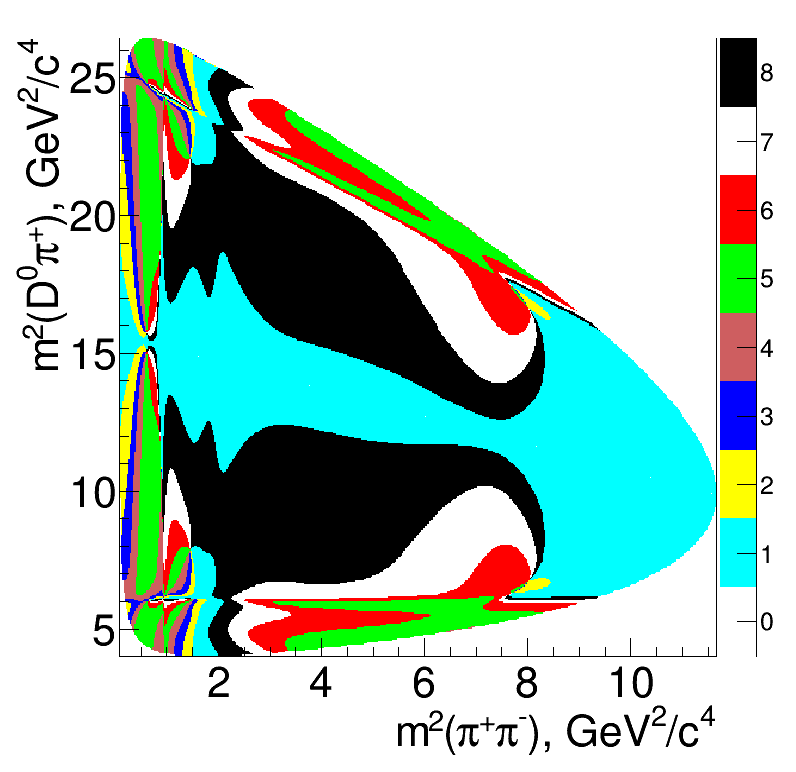
\includegraphics[width=0.8\textwidth]{d0pipi_binning2_rotated}
 \subcaption{}
 \label{fig:bdbpp-bins}
\end{minipage}
\begin{minipage}[b]{0.5\textwidth}
 \centering
  \includegraphics[width=0.8\textwidth]{CS_bdpp_v4}
 \subcaption{}
 \label{fig:csj}
\end{minipage}
 \caption{а) Равномерное по фазе разбиение диаграммы Далица распада \bdbpp, полученное на основе упрощенной версии модели, опубликованной в работе~\cite{kuzmin_model}, и б) значения параметров $c_j$ и $s_j$, полученные с помощью этой модели, (синие круги).  Красные квадраты показывают пример измерения и ожидаемую точность при измерении параметров $c_j$ и $s_j$ в эксперименте \belleii.}
 \label{fig:bdbpp}
\end{figure}

Полученные значения параметров $k_j$, $c_j$ и $s_j$ использованы для генерирования событий в соответствии с оценками из таблицы~\ref{tab:yield}.  Сгенерированные события использовались для определения величин параметров \pphi, $c_j$ и $s_j$ методом максимального правдоподобия.  Полученные значения статистической неопределенности для параметра \pphi приведены в таблице~\ref{tab:precision}.  На рисунке~\ref{fig:csj} показан результат определения величины параметров $c_j$ и $s_j$, соответствующий размеру выборки, ожидаемому в эксперименте \belleii.

\begin{table}[H]
 \centering
 \caption{Результаты численных экспериментов: статистическая неопределенность при модельно-независимом измерении параметра \pphi в распадах \bdbpp и \bdsth с последующими переходами $D$-мезона в \cpconj-собственные состояния и состояние \kspp.  Результаты были получены для значения параметра $\pphi=23\grad$.}
 \label{tab:precision}
\begin{tabular}{lcc}
 \hline\hline
 \multirow{2}{*}{Тип событий}& \multicolumn{2}{c}{$\delta\pphi$ (град.)} \\
                          & \belle          & \belleii \\% & LHCb (RI) & LHCb (RII) & LHCb (Upg)\\
 \hline
 \bdbpp                   & $ 7.6\grad$ & $1.2\grad$\\ % & $8.2\grad$ & $7.7\grad$ & $1.9\grad$ \\
 \bdbpp (симм. области)   & $10\grad$   & $1.5\grad$\\ % & $16\grad$  & $10\grad$ & $2.7\grad$ \\
 \bdsth                   & $ 4.4\grad$ & $0.7\grad$\\ % & --- & --- & --- \\
 \hline\hline
 \end{tabular}
\end{table}

Полученные результаты позволяют сделать несколько выводов.  Точность модельно-независимого измерения параметра \pphi в распадах \bdbpp примерно в~$1.5$ раз хуже, чем в распадах~\bdsth.  Симметризация областей на диаграмме Далица распада \bdbpp приводит к значительному уменьшению статистической чувствительности метода; эта модификация может быть выбрана только из соображений сложных фоновых условий в конкретном измерении.  
Можно ожидать, что данные эксперимента \belleii позволят выполнить модельно-независимое измерение параметра \pphi в переходах \btocud с точностью лучше~$1\grad$.  Этот результат будет служить важным инструментом для проверки механизма \km и ограничения вкладов НФ.

\section{Разбиение фазового пространства в пределе большой статистики}\label{sec:big-data}
Завершая обсуждение модельно-независимого подхода к анализу многочастичных распадов, кратко рассмотрим вопрос об оптимизации разбиения фазового пространства в условиях большого количества экспериментальных данных.  В работах~\cite{Bondar2008,CLEO_phases} рассматривался вопрос об оптимизации формы областей при заданном их количестве $2\mcn$.  Процедуры оптимизации, предложенные в этих работах, основаны на использовании модели распада и дают желаемый результат только при условии адекватности модели.

Более прямолинейный путь приближения к предельной статистической чувствительности метода состоит в увеличении количества областей, на которые разбивается фазовое пространство распада \dnkpp.  При этом, количество областей разумно увеличивать только до тех пор, пока размер области больше или порядка экспериментального разрешения для переменных Далица (которое для $B$-фабрик близко к $2\times 10^{-3}\gev^{2}/c^{4}$).  Этот предел приблизительно соответствует $4\times 10^5$ областям.  Учитывая, что на Супер-Чарм-Тау-фабрике со светимостью $10^{35}\lumi$ число событий с распадом обоих $D$-мезонов в \kspp может достигать $10^6$ событий, число областей фазового пространства может достигать нескольких тысяч.

При $\mcn\gtrsim 100$ могут возникнуть сложности вычислительного характера, поскольку при измерении параметров \ci и \si необходимо решать систему из $\mcn^2$ нелинейных уравнений относительно $2\mcn$ неизвестных (смотрите пункт~\ref{sec:cs_measurement}).  Одна из возможных процедур, свободная от сложностей такого рода, состоит в измерении параметров \ci и \si в два этапа.  На первом этапе реализуется описанная в пункте~\ref{sec:cs_measurement} процедура для небольшого $\mcn_0$, например, равного $8$.  Затем, при анализе когерентных  распадов $\ep\to(\kspp)_D(\kspp)_D$, для одной из диаграмм Далица используется $\mcn_0$, а для другой --- большое \mcn.  При такой процедуре система уравнений разбивается на $\mcn$ независимых систем, каждая из которых содержит $4\mcn_0$ уравнений ($2\mcn_0$ уравнений для каждой пары симметричных областей мелкого разбиения и двух неизвестных параметров~\ci и~\si).

При наличии Супер-Чарм-Тау-фабрики, вероятно, статистическая точность определения параметра \gphi будет определяться числом событий \bdk, \dkpp в экспериментах \belleii и \lhcb (можно ожидать порядка $10^5$ событий).  Максимальное число областей фазового пространства распада \dnkpp при этом может достигать нескольких тысяч, а экспериментальное разрешение для переменных Далица еще не будет ограничивающим фактором.

Можно ожидать, что при разбиении фазового пространства на $10^3$ и более областей, форма каждой области уже не будет иметь существенного значения, а статистическая точность метода будет близка к точности модельно-зависимого измерения.
%Помимо этого, остается открытым вопрос о существовании правила разбиения фазового пространства, которое в общем случае приводило бы к лучшей статистической чувствительности, чем правило~\eqref{eq:uniph}.  


